\documentclass[conference]{IEEEtran}
\usepackage[UTF8,scheme=plain,fontset=windows]{ctex}
\usepackage{amsmath,amssymb}
\usepackage{graphicx}
\usepackage{booktabs}
\usepackage{multirow}
\usepackage{array}
\usepackage{cite}
\usepackage{url}
\usepackage{xcolor}
\usepackage{stfloats}
\usepackage{float}
\graphicspath{{figures/}}

\title{面向概念证据缺口的支持约束概念可达性认知诊断}

\author{
\IEEEauthorblockN{匿名作者}
\IEEEauthorblockA{匿名单位\\
Email: anonymous@example.com}
}

\begin{document}
\maketitle

\begin{abstract}
认知诊断旨在根据学生历史作答推断其对知识概念的掌握状态。从教育测量视角看，诊断模型需要把历史作答与当前目标概念判断联系起来。现有神经认知诊断和图认知诊断模型通常依赖学生--题目响应日志和 Q 矩阵进行预测，但在真实学习平台中，学生历史并不总是直接覆盖当前题目涉及的目标概念，导致目标概念缺少直接历史支持。本文提出面向概念覆盖不足场景的概念可达性认知诊断框架。该框架包含概念可达图（Concept Reachability Graph, CRG）和学习者条件化可达性过滤器（Learner-Conditioned Reachability Filter, LCRF）。CRG 使用训练集中的题内概念共现、序列转移和自保持关系构造概念可达图，为目标概念提供固定支持集；LCRF 在该支持集内根据学生掌握度、近期表现和历史计数重排支持概念的后验权重。三个真实数据集上的实验表明，该框架在整体预测上保持竞争性能；进一步分析显示，CRG 能从学生历史概念中检索目标概念，CRG/LCRF 的收益主要集中在目标概念直接覆盖不足但仍存在候选支持的场景中。
\end{abstract}

\begin{IEEEkeywords}
认知诊断，概念证据缺口，概念可达图，支持约束，学习者条件化过滤
\end{IEEEkeywords}

\section{引言}
认知诊断（Cognitive Diagnosis, CD）是智能教育系统中的基础任务，目标是根据有限作答证据推断学生对知识概念的掌握状态。证据中心评估强调，测评结论应由观测证据、认知状态和解释规则共同支撑~\cite{pellegrino2001knowing,mislevy2003structure}。因此，一个可靠的诊断模型应当回答：当前预测依据了哪些可观察作答，这些作答如何支持目标概念上的掌握判断。诊断结果进一步服务于个性化练习推荐、补救学习、学习路径规划和自适应测试；模型需要在保持预测能力的同时，给出概念层面的支持来源。

在真实学习平台中，学生历史作答往往只覆盖部分概念。当前题目涉及的目标概念可能从未出现在该学生历史中，或者只有极少量直接观测。此时，模型虽然仍可给出预测，但从学生已有作答到目标概念掌握状态之间缺少明确的概念层支持。本文将这一现象称为\emph{概念证据缺口}：目标概念需要被诊断，但学生历史中缺少直接概念证据，模型必须从相关历史概念和训练日志中的概念关系中寻找支撑。

现有神经 CDM 和图 CDM 多依赖学生--题目响应、Q 矩阵或异构图传播，但通常把两个层次的问题压缩到同一个表示学习过程。第一层是\emph{支持集构造}：当目标概念没有在学生历史中直接出现时，模型需要从学生已经练习过的相关概念出发，借助训练日志中的概念关系找到候选支持概念。第二层是\emph{学生状态过滤}：同一组候选支持概念并不一定适合所有学生，模型还需要根据当前学生的掌握度、近期表现和历史可靠性判断哪些支持更可信。

这一区分对真实学习平台尤其重要。若只依赖题内多概念共现，单概念题占比很高的数据集中概念关系图容易退化为自连接，目标概念和历史概念之间缺少可用连接；若只依赖学生或题目嵌入，模型可能仍能拟合正确率，却难以说明目标概念判断主要受到哪些历史概念支撑。从教育诊断角度看，把历史概念连接到目标概念，相当于为当前掌握判断寻找可解释的先前表现来源；这种连接可以来自同题共现，也可以来自学习日志中观察到的经验学习顺序。因此，概念证据缺口需要一种同时具备概念支持集构造和学生状态过滤能力的诊断机制。

本文提出 CRG/LCRF 两阶段框架。CRG 建模目标概念是否存在训练日志支持的候选支持概念；LCRF 在固定 CRG 支持集内估计这些支持概念对当前学生的后验权重。二者分别对应支持集构造与支持集内个性化过滤。

\begin{figure*}[!t]
  \centering
  
\includegraphics[width=0.96\textwidth]{fig1_problem_concept_evidence_gap.png}
  \caption{概念证据缺口问题。当前目标概念可能没有被学生历史直接覆盖，导致从历史作答到目标概念掌握状态之间缺少直接证据。CRG 用训练集可观察关系提供候选支持概念，LCRF 在固定支持集内根据学生状态重排后验权重。}
  \label{fig:concept-gap}
\end{figure*}

如图~\ref{fig:concept-gap} 所示，学生历史中已有概念提供有限的历史线索，但目标概念 \(c_q\) 未必出现在历史概念集合中。CRG 利用训练日志中的经验关系把历史概念连接到目标概念，其中 sequence transition 表示日志中观察到的学习顺序，而非严格先修关系。LCRF 则在 CRG 给出的固定 support 内进行个性化后验重排，使支持概念的权重随学生状态变化而变化。换言之，CRG 判断哪些概念可以作为目标概念的候选支持，LCRF 判断这些候选支持对当前学生的相对权重。该设计与学习支架思想一致：全局可用的概念支持只有与学生当前状态匹配时，才更适合作为局部预测信号。

本文贡献如下：
\begin{itemize}
  \item 提出概念证据缺口问题，将目标概念直接证据不足的诊断转化为历史概念到目标概念的支持集构造问题。
  \item 提出 CRG，仅使用训练阶段的题内共现、序列转移和自保持证据构造全局概念支持集。
  \item 提出 LCRF，在固定 CRG 支持集内根据学生状态重排支持概念的后验权重，实现支持集约束的个性化诊断。
\end{itemize}

\section{相关工作}
\subsection{认知诊断模型}
传统认知诊断模型通常建立在心理测量理论之上，例如 IRT、MIRT 和 DINA~\cite{lord1980irt,reckase2009mirt,delatorre2009dina,templin2006cdm}。它们通过预设交互函数描述学生能力、题目难度和作答结果之间的关系，具有较强解释性，但表达能力有限。FuzzyCD 等方法进一步扩展了传统诊断模型对模糊掌握状态的刻画~\cite{liu2018fuzzycd}。神经认知诊断模型使用神经网络建模复杂的学生--题目交互，使模型能够从大规模作答数据中学习非线性诊断函数~\cite{wang2020ncdm}。NCDM、KaNCD 等方法将学生、题目和概念表示映射到连续空间中~\cite{wang2020ncdm,wang2022kscd}，RCD、SCD、ORCDF 等图式方法进一步利用学生--题目--概念关系提升表示能力~\cite{gao2021rcd,wang2023scd,qian2024orcdf}。

这些方法主要从作答结果中估计掌握状态，但较少显式区分目标概念是否已被学生历史直接覆盖。本文将关注点放在目标概念与学生历史概念之间缺少直接概念证据的场景，分析模型如何构造可用的概念支持。

\subsection{图认知诊断与概念关系建模}
图认知诊断模型通过学生--题目图、题目--概念图或异构图传播建模高阶关系。相关工作表明，图结构可以提升学生和题目的表示能力，并有助于建模概念、题目和学生之间的依赖关系~\cite{kipf2017gcn,velickovic2018gat,hamilton2017graphsage,he2020lightgcn,su2022gcdm}。与此同时，图结构也需要明确边的来源、方向和作用方式。已有研究从学生--题目边的异质性、不确定性和噪声角度分析图传播问题~\cite{wang2024uncertaintycd,shao2025isgcd,zhang2026ncdla}；本文则从目标概念缺少直接历史覆盖时的概念支持来源出发，构造由训练日志关系约束的概念可达图，并在固定支持集内进行学习者条件化过滤。

与 RCD、SCD、ORCDF 等直接在学生--题目或异构图上传播表示的方法不同，CRG 面向概念层面的支持集构造，重点在于为目标概念选择可用的候选概念集合~\cite{gao2021rcd,wang2023scd,qian2024orcdf}。与关注学生--题目边不确定性的 ISG-CD 不同，本文从题内共现、序列转移和自保持中构造概念间关系，并将个性化限制在固定支持集内~\cite{shao2025isgcd}。

\subsection{稀疏证据与可靠诊断}
现有研究已从冷启动学生/题目、非随机缺失响应、噪声交互和不可靠图边等角度研究认知诊断中的数据不足问题。KCD 和 LRCD 等方法利用文本语义或语言表示缓解冷启动、开放环境或跨域诊断问题~\cite{dong2025kcd,liu2025lrcd}；DBCD、HeckmanCD 和公平性认知诊断工作从非随机缺失、选择偏差与反事实建模角度分析学生选择性作答带来的偏差~\cite{yang2026dbcd,han2024heckmancd,zhang2024faircd,zhang2024causalcdf}；NCDLA 和 DisenGCD 从噪声、低秩结构或解耦图表示角度研究图认知诊断的鲁棒性~\cite{zhang2026ncdla,yang2024disengcd}。与此同时，语言学习和对话式学习诊断进一步拓展了 CD 在开放文本和交互式教育场景中的应用~\cite{ma2024languagecd,yao2026parld}。本文关注目标概念层面的证据缺口：学生可能拥有一定长度的历史作答记录，但这些记录并不直接包含当前题目所需概念。因此，模型需要判断目标概念能否由历史概念通过训练日志中的概念关系获得支持，并进一步判断该支持集是否适合当前学生。CRG 和 LCRF 分别对应这两个层次：前者构造全局可达支持集，后者在固定支持集内建模学习者条件化后验分布。

\subsection{教育测量视角与学习支架}
教育测量研究强调，诊断结论应由可观察作答与解释规则共同支撑~\cite{pellegrino2001knowing,mislevy2003structure}。在这一视角下，目标概念缺少直接历史覆盖体现了历史作答与当前概念之间的联系不足。CRG 中的序列关系可与学习进阶研究中的经验发展路径相呼应，但本文不将其解释为严格先修关系~\cite{corcoran2009learning}。LCRF 则与最近发展区、学习支架和掌握学习思想一致：全局可用支持需要根据学生当前状态进行选择和调节~\cite{vygotsky1978mind,wood1976tutoring,bloom1968learning}。因此，CRG/LCRF 的目标是在直接覆盖不足时补充概念支持和学生条件化过滤。

\section{问题定义}
设学生、题目和概念集合分别为 \(\mathcal{U}\)、\(\mathcal{E}\) 和 \(\mathcal{C}\)。题目--概念矩阵 \(Q\) 描述每道题涉及的概念，学生作答日志 \(\mathcal{R}\) 由学生、题目和二值作答结果组成。给定学生 \(u\) 在时间 \(t\) 的 query exercise，记 \(H_{u,t}\) 为该学生此前作答历史中出现过的概念集合。

本文使用两个诊断量刻画 query 的覆盖条件。直接覆盖 \(D_{u,t}(c)\) 表示目标概念 \(c\) 是否已经出现在 \(H_{u,t}\) 中；CRG reachability 表示目标概念是否能在 CRG 给出的固定支持集 \(S_A(c)\) 中获得候选支持概念。若 \(D_{u,t}(c)=0\)，模型缺少该学生在目标概念上的直接历史表现；若同时存在 CRG reachability，则目标概念仍可能由学生历史中的相关概念通过训练阶段概念关系获得支持。

这两个量只用于刻画样本的覆盖条件，而不是限制预测任务本身。模型仍在完整作答样本上训练与评估；覆盖条件分析只用于观察模型在 direct-unseen、bridgeable 或 high-score 等子场景中的表现。概念可达图由训练阶段可观测的概念关系估计，并在验证与测试阶段保持固定。

\section{概念证据缺口现象}
\begin{figure}[!t]
  \centering
  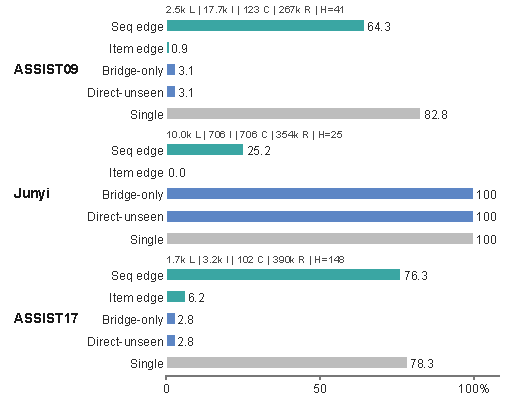
\includegraphics[width=0.98\columnwidth]{fig_dataset_evidence_profiles.pdf}
  \caption{数据集覆盖缺口画像。蓝色条表示直接覆盖条件，青色条表示可用路线来源，灰色条表示单概念题比例；每个卡片顶部给出学生数（L）、题目数（I）、概念数（C）、作答数（R）和历史长度中位数（H）。}
  \label{fig:dataset-profile}
\end{figure}

图~\ref{fig:dataset-profile} 展示三个数据集的规模与概念覆盖缺口画像，也作为本文的问题存在性分析。Direct-unseen rate 表示测试样本中目标概念从未出现在该学生历史概念集合中的比例；bridge-only rate 表示这些 direct-unseen 样本中，目标概念仍可通过 CRG 支持集与历史概念相连的比例。二者分别刻画“缺少直接概念覆盖”和“仍存在候选支持概念”两个条件。三组数据体现了不同的覆盖条件：Junyi 无题内共现但可由序列关系补充；ASSIST09 和 ASSIST17 是题内证据较稀疏但序列证据较强的平衡场景。

Junyi 没有题内概念共现，但 direct-unseen rate 与 bridge-only rate 均很高，说明目标概念经常缺少学生历史中的直接覆盖，却可以通过训练日志中的序列关系获得候选支持。ASSIST09 和 ASSIST17 更接近常规 benchmark，少量题内共现与较强序列关系共同存在。这里的概念共现指同一道题同时涉及多个概念，例如一道代数题可能同时考查“移项”和“一元方程求解”，这两个概念就在该题中共同出现。上述差异说明，概念证据缺口需要同时考虑题内多概念共现和训练日志中的经验学习顺序。数据画像先验证目标场景是否真实存在，后续检索和分组预测实验再检验 CRG/LCRF 是否能在该场景中提供有效支持。

\section{方法}
\subsection{框架总览}
本文框架包括两个递进组件：CRG 和 LCRF。CRG 负责构造全局概念可达图，用于形成固定支持集；LCRF 负责在该支持集上进行学习者条件化后验过滤。计算过程分为四步。首先，训练阶段概念关系估计全局可达图 \(A_{\mathrm{CRG}}\)。其次，\(A_{\mathrm{CRG}}(c,:)\) 为目标概念 \(c\) 选择固定支持集 \(S_A(c)\)。随后，LCRF 结合 \(S_A(c)\) 与学生状态 \(\mathbf{x}_{u,t}\) 生成支持概念后验分布 \(P_{\mathrm{LCRF}}(k|u,t,c)\)。最后，诊断预测头使用该后验分布得到作答概率 \(\hat r_{u,e}\)。

\begin{figure*}[!t]
  \centering
  
\includegraphics[width=0.96\textwidth]{fig2_crg_lcrf_architecture.png}
  \caption{CRG/LCRF 框架。CRG 使用训练集中的题内概念共现、序列转移和自保持关系构造全局概念可达图，并为目标概念给出固定 support。LCRF 在该 support 内根据学生 mastery、近期表现和历史计数重排支持概念的 posterior weight，最后用于目标概念掌握度预测。}
  \label{fig:framework}
\end{figure*}

图~\ref{fig:framework} 展示了 CRG/LCRF 的整体机制路径。CRG 从训练阶段可观测关系中构造概念可达图，关系包括题内共现、序列转移、自保持以及 source/receiver reliability。随后，CRG 为当前 query concept 给出固定支持集 \(S_A(c)\)。LCRF 根据 query mastery、recent mastery、support-concept mastery、readiness gap 和 support count 等学生状态信号，对同一支持集内的后验权重进行个性化重排。

\subsection{概念可达图 CRG}
CRG 是训练集关系约束的概念支持图，用来为目标概念寻找候选支持概念。给定两个概念 \(a,b\)，题内共现、序列转移和自保持信号定义为：
\[
\begin{aligned}
M^{item}_{a,b}
&=\sum_{e\in \mathcal{E}^{tr}} Q_{e,a}Q_{e,b}\mathbb{I}[a\neq b],\\
M^{seq}_{a,b}
&=\sum_{u,t}
\mathbb{I}[a\in C(e_{u,t})]\,
\mathbb{I}[b\in C(e_{u,t+1})],\\
M^{self}_{a,b}
&=\mathbb{I}[a=b].
\end{aligned}
\]
\(M^{item}\) 只在题内多概念共现可用时提供概念关系；自保持由 \(M^{self}\) 单独建模，因此题内共现只刻画不同概念之间的同题关系。\(M^{seq}\) 表示训练日志中的经验学习顺序，而非严格先修关系，这与学习进阶研究中强调经验发展路径而非单一因果先修的观点一致~\cite{corcoran2009learning}。\(M^{self}\) 保留目标概念自身状态。

从教育诊断角度看，把历史概念连接到目标概念，相当于为当前判断寻找可解释的先前表现支撑；这种支撑来自学生曾练习过的相关概念和训练日志中的经验学习顺序，而不是确定的课程先修链。为使不同来源处在可比较尺度上，CRG 将计数证据转换为概念关系分数：
\[
\begin{aligned}
s_{item}(a,b)&=\lambda_{item}\phi(M^{item}_{a,b}),\\
s_{seq}(a,b)&=\lambda_{seq}\phi(M^{seq}_{a,b}),\\
s_{self}(a,b)&=\lambda_{self}M^{self}_{a,b}.
\end{aligned}
\]
三类分数与接收端偏置 \(b_b\) 合成为总关系分数：
\[
s(a,b)=s_{item}(a,b)+s_{seq}(a,b)+s_{self}(a,b)+b_b .
\]
归一化之前，CRG 先收集至少由一种训练阶段关系支持的候选概念：
\[
\mathcal{N}(a)
=
\{b\mid
M^{item}_{a,b}
+M^{seq}_{a,b}
+M^{self}_{a,b}>0
\}.
\]
随后在候选集合 \(\mathcal{N}(a)\) 上进行行归一化：
\[
A_{\mathrm{CRG}}(a,b)
=\operatorname{softmax}_{b\in \mathcal{N}(a)}
\left(s(a,b)/\tau\right).
\]
其中 \(\tau\) 控制关系分布的平滑程度。对目标概念 \(c\)，固定支持集由 top-\(K\) 邻居概念得到：
\[
S_A(c)=
\operatorname{TopK}_{k\in \mathcal{N}(c)}
A_{\mathrm{CRG}}(c,k).
\]
其中 \(\mathcal{N}(a)\) 是候选概念集合，\(S_A(c)\) 是 LCRF 针对目标概念 \(c\) 使用的固定支持集。该集合是后续 LCRF 可使用的候选概念范围，也构成 CRG 和 LCRF 的模块边界。

\subsection{学习者条件化可达性过滤器 LCRF}
LCRF 是支持集约束的个性化后验过滤器。CRG 给出全局支持集，但同一组支持概念对不同学生不一定同等适用。受学习支架与最近发展区思想启发，LCRF 将全局候选支持进一步过滤为适合当前学生状态的局部支持~\cite{vygotsky1978mind,wood1976tutoring}。

LCRF 首先把 CRG 关系概率写成先验 logit：
\[
z^{prior}_{c,k}=\log A_{\mathrm{CRG}}(c,k).
\]
随后，学生状态产生局部校正项：
\[
\begin{aligned}
\Delta_{u,t,c,k}&=f_{\theta}(\mathbf{x}_{u,t,c,k}),\\
z^{state}_{u,t,c,k}&=\alpha_{u,t,c}\Delta_{u,t,c,k}.
\end{aligned}
\]
其中 \(\mathbf{x}_{u,t,c,k}\) 包含 query concept 与 support concept 的掌握度 \(m\)、近期表现 \(\rho\)、历史计数或可靠性 \(n\)。二者相加后在固定支持集内归一化：
\[
\begin{aligned}
z_{u,t,c,k}
&=z^{prior}_{c,k}+z^{state}_{u,t,c,k},\\
P_{\mathrm{LCRF}}(k|u,t,c)
&=\operatorname{softmax}_{k\in S_A(c)}(z_{u,t,c,k}).
\end{aligned}
\]
由于 softmax 被限制在 \(S_A(c)\) 内，LCRF 调整的是固定 CRG 支持集上的后验权重。预测时，后验分布用于聚合支持概念的掌握度：
\[
\begin{aligned}
\tilde{m}_{u,t}(c)=&
(1-\gamma)m_{u,t}(c)\\
&+\gamma
\sum_{k\in S_A(c)}
P_{\mathrm{LCRF}}(k|u,t,c)m_{u,t}(k).
\end{aligned}
\]

\subsection{预测与优化}
最终，融合支持概念后的掌握表示被送入诊断预测头得到作答概率 \(\hat r_{u,e}\)。模型使用训练作答上的二分类交叉熵进行优化。消融实验中的 w/o CRG 对应移除 \(A_{\mathrm{CRG}}\) 和固定支持集，w/o LCRF 对应移除学生状态校正项 \(z^{state}_{u,t,c,k}\)。

\section{实验}
实验围绕方法中的两个操作组织。首先，主预测性能比较 CRG-LCRF 与代表性 CD baseline，验证模型是否具备整体竞争力。其次，概念检索实验分析直接覆盖不足时，训练日志中的概念关系能否为目标概念提供候选支持。最后，模块消融、支持集扰动、学习者状态反事实和同题个案进一步分析支持集构造与学生状态过滤如何影响预测。

\subsection{实验设置}
实验使用三个公开认知诊断数据集：ASSIST09、Junyi 和 ASSIST17~\cite{assistments2009,heffernan2017assistments,assistments2017,choi2020ednet}。其中 ASSIST09 与 ASSIST17 是 ASSISTments 系列中常用的简称，Junyi 来自大规模在线学习平台。图~\ref{fig:dataset-profile} 给出了预处理后的学生数、题目数、概念数、作答数和覆盖统计。所有数据集均使用既定 train/validation/test split；CRG 由训练阶段可观测关系估计，并在验证和测试阶段保持固定。评价指标包括 AUC、ACC、RMSE 和 BCE，其中 AUC 作为主要预测指标，BCE 用于观察覆盖条件子场景中的概率预测变化。Baseline 覆盖传统与深度方法（IRT、DINA、NeuralCD）、图式方法（LightGCN、KaNCD、RCD）以及解耦表示方法（SCD）~\cite{lord1980irt,delatorre2009dina,wang2020ncdm,he2020lightgcn,wang2022kscd,gao2021rcd,wang2023scd}。

\subsection{主预测性能}
\begin{table*}[!t]
\centering
\caption{主数据集上的整体预测性能。}
\label{tab:main-performance}
\small
\setlength{\tabcolsep}{5pt}
\begin{tabular}{llcccccc}
\toprule
\multirow{2}{*}{方法类别} & \multirow{2}{*}{模型} &
\multicolumn{2}{c}{ASSIST09} & \multicolumn{2}{c}{Junyi} & \multicolumn{2}{c}{ASSIST17}\\
\cmidrule(lr){3-4}\cmidrule(lr){5-6}\cmidrule(lr){7-8}
& & AUC & ACC & AUC & ACC & AUC & ACC\\
\midrule
Traditional \& Deep & IRT & 0.7415 & 0.7132 & 0.7789 & 0.7392 & 0.7238 & 0.6561\\
Traditional \& Deep & DINA & 0.7482 & 0.7158 & 0.7795 & 0.7421 & 0.7259 & 0.6625\\
Traditional \& Deep & NeuralCD & 0.7523 & 0.7228 & 0.7812 & 0.7472 & 0.7320 & 0.6700\\
Graph-based & LightGCN & 0.7593 & 0.7256 & 0.7832 & 0.7502 & 0.7512 & 0.6813\\
Graph-based & KaNCD & 0.7640 & 0.7315 & 0.7885 & 0.7556 & 0.7640 & 0.7315\\
Graph-based & RCD & 0.7685 & 0.7330 & 0.8087 & 0.7685 & 0.7676 & 0.6953\\
Disentangled & SCD & 0.7701 & 0.7321 & 0.8134 & 0.7726 & 0.7753 & 0.7028\\
\textbf{Ours} & \textbf{CRG-LCRF} & \textbf{0.7783} & \textbf{0.7407} & \textbf{0.8291} & 0.7688 & \textbf{0.7847} & \textbf{0.7151}\\
\bottomrule
\end{tabular}
\end{table*}

表~\ref{tab:main-performance} 给出三个主数据集上的整体预测性能。CRG-LCRF 在 Junyi 上取得最高 AUC，说明在无题内共现但存在序列关系的场景中，显式概念支持能带来更强预测能力。在 ASSIST09 和 ASSIST17 上，CRG-LCRF 与代表性图式和解耦模型保持竞争水平。该主表用于说明模型具备稳定预测基础；后续实验进一步分析概念证据缺口子场景中的收益来源。

从整体结果看，CRG-LCRF 明显优于传统方法和基础图式方法。在 Junyi 上，CRG-LCRF 相比 SCD 提升 0.0157 AUC，体现了无题内共现条件下 sequence support 的价值。在 ASSIST09 和 ASSIST17 上，CRG-LCRF 分别高于 SCD 0.0082 和 0.0094 AUC，说明其整体预测能力具备竞争性。除整体预测性能外，CRG-LCRF 还提供了可分解的概念支持与 learner-conditioned filtering，便于在覆盖条件子场景中定位收益来源。

\subsection{概念检索与覆盖条件预测}
本节把两个主问题实验放在一起分析。首先，history-to-query retrieval 检验 CRG 能否从学生历史概念中检索当前目标概念。给定学生历史概念集合 \(H_{u,t}\) 与 query concept \(c\)，我们使用 CRG 关系分数对候选概念排序，并评估真实 query concept 的 Hit@5、Hit@10、NDCG@10 和 MRR。随后，coverage-conditioned prediction 进一步分析这些候选支持是否在 direct-unseen-bridgeable、weak-direct 和 high-score 等子场景中转化为预测收益。

\begin{figure}[H]
  \centering
  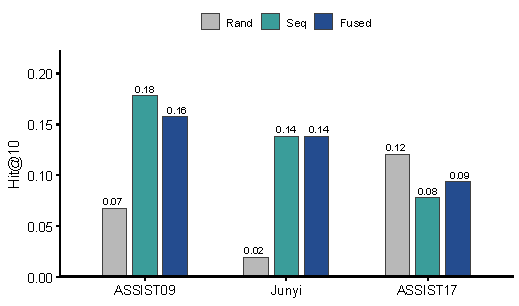
\includegraphics[width=0.98\columnwidth]{fig4_history_to_query_retrieval.pdf}
  \caption{History-to-query 概念检索结果。图中比较 random、seq-only 与 fused CRG 在 direct-unseen-bridgeable 查询上的 Hit@10；ASSIST17 作为该检索设置下较不有利的对照数据集保留。}
  \label{fig:history-to-query}
\end{figure}

\begin{figure}[H]
  \centering
  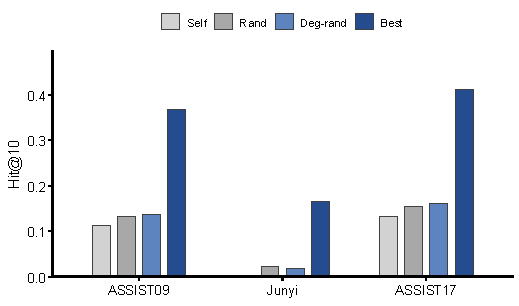
\includegraphics[width=0.98\columnwidth]{fig5_heldout_transition_retrieval.pdf}
  \caption{全局留出概念转移检索结果。Best CRG 表示每个数据集上表现最好的 CRG 路线来源，用于比较训练阶段概念关系是否能恢复留出的概念转移。}
  \label{fig:heldout}
\end{figure}

图~\ref{fig:history-to-query} 评估给定学生历史概念集合时，训练日志中的概念关系能否检索当前 query concept。在 direct-unseen-bridgeable 子场景中，ASSIST09 的 random Hit@10 为 0.0673，而 seq-only 和 fused CRG 分别达到 0.1781 和 0.1574；Junyi 的 random Hit@10 为 0.0191，而 seq-only 和 fused CRG 均达到 0.1379。该结果表明，训练阶段概念关系可以在目标概念缺少直接历史覆盖时提供候选支持。ASSIST17 在该检索任务上的表现模式不同，因此这里将其作为对照，而不是将该任务写成三个数据集上的一致正结果。

图~\ref{fig:heldout} 从全局概念转移恢复角度补充验证 CRG。Best CRG 在三个数据集上均高于 self-only、random 和 degree-random，说明训练阶段概念关系可以恢复留出的概念转移。该结果与 history-to-query 检索互补：前者观察全局概念转移，后者观察学生历史概念到当前目标概念的检索。

覆盖条件预测不再额外放大表，而是在正文中报告主要趋势。ASSIST09 的 direct-unseen-bridgeable、低直接覆盖与 high-score 子场景中，Full 相对 w/o CRG 和 w/o LCRF 均保持更低 BCE，其中 direct-unseen-bridgeable 子场景的 BCE 差值分别为 0.0219 和 0.0382。ASSIST17 的 high-score 与低直接覆盖子场景中，Full 相比 w/o CRG 的 AUC 提升约为 0.0151，BCE 差值也保持为正；相比 w/o LCRF 时，AUC 差异较小，但 BCE 仍有改善。在 Junyi 中，检索结果与数据现象更突出，预测层收益主要体现为候选支持场景下的补充信号。

这两个结果合在一起说明，概念证据缺口场景需要结合分组分析理解模型行为。概念检索先验证训练阶段概念关系能否为目标概念提供候选支持；覆盖条件预测进一步显示，这类候选支持在 direct-unseen、high-score 或低直接覆盖样本上更容易转化为概率预测收益。因此，后续模块分析重点观察模型是否实际使用 CRG 支持集，以及 LCRF 是否根据学生状态改变支持集内的后验分布。

\subsection{模块消融}
\begin{table}[H]
\centering
\caption{三个数据集上的模块消融结果。}
\label{tab:ablation}
\small
\setlength{\tabcolsep}{3.2pt}
\begin{tabular}{llccc}
\toprule
数据集 & 指标 & Full & w/o CRG & w/o LCRF\\
\midrule
\multirow{3}{*}{ASSIST09}
& AUC  & \textbf{0.7783} & 0.7671 & 0.7634\\
& ACC  & \textbf{0.7407} & 0.7320 & 0.7309\\
& RMSE & \textbf{0.4178} & 0.4222 & 0.4247\\
\midrule
\multirow{3}{*}{Junyi}
& AUC  & \textbf{0.8291} & 0.8278 & 0.8286\\
& ACC  & 0.7688 & 0.7691 & \textbf{0.7701}\\
& RMSE & 0.4008 & 0.4011 & \textbf{0.3994}\\
\midrule
\multirow{3}{*}{ASSIST17}
& AUC  & \textbf{0.7847} & 0.7647 & 0.7829\\
& ACC  & \textbf{0.7151} & 0.6973 & 0.7132\\
& RMSE & \textbf{0.4321} & 0.4413 & 0.4359\\
\bottomrule
\end{tabular}
\end{table}

表~\ref{tab:ablation} 展示三个数据集上的模块消融结果。Full 表示完整模型；w/o CRG 移除全局概念可达图；w/o LCRF 保留 CRG 但移除学习者条件化过滤。

完整模型在 ASSIST09 和 ASSIST17 上取得最高 AUC，相比 w/o CRG 分别提升 1.12\% 和 2.00\%。移除 LCRF 在 ASSIST09 上带来更明显下降，而在 Junyi 与 ASSIST17 的直接模块删除设置下影响较小。该结果说明，CRG 提供主要的候选支持信号；LCRF 的作用在学习者状态替换实验中表现得更直接。

\subsection{CRG 支持集扰动分析}
概念检索评估 CRG 的恢复能力；支持集扰动进一步分析预测对支持集的敏感性。我们在推理阶段替换或破坏 CRG 支持集，并观察预测性能变化。对照包括证据支持集替换、度匹配随机支持集、序列打乱支持集和 self-only fallback。

\begin{figure}[H]
  \centering
  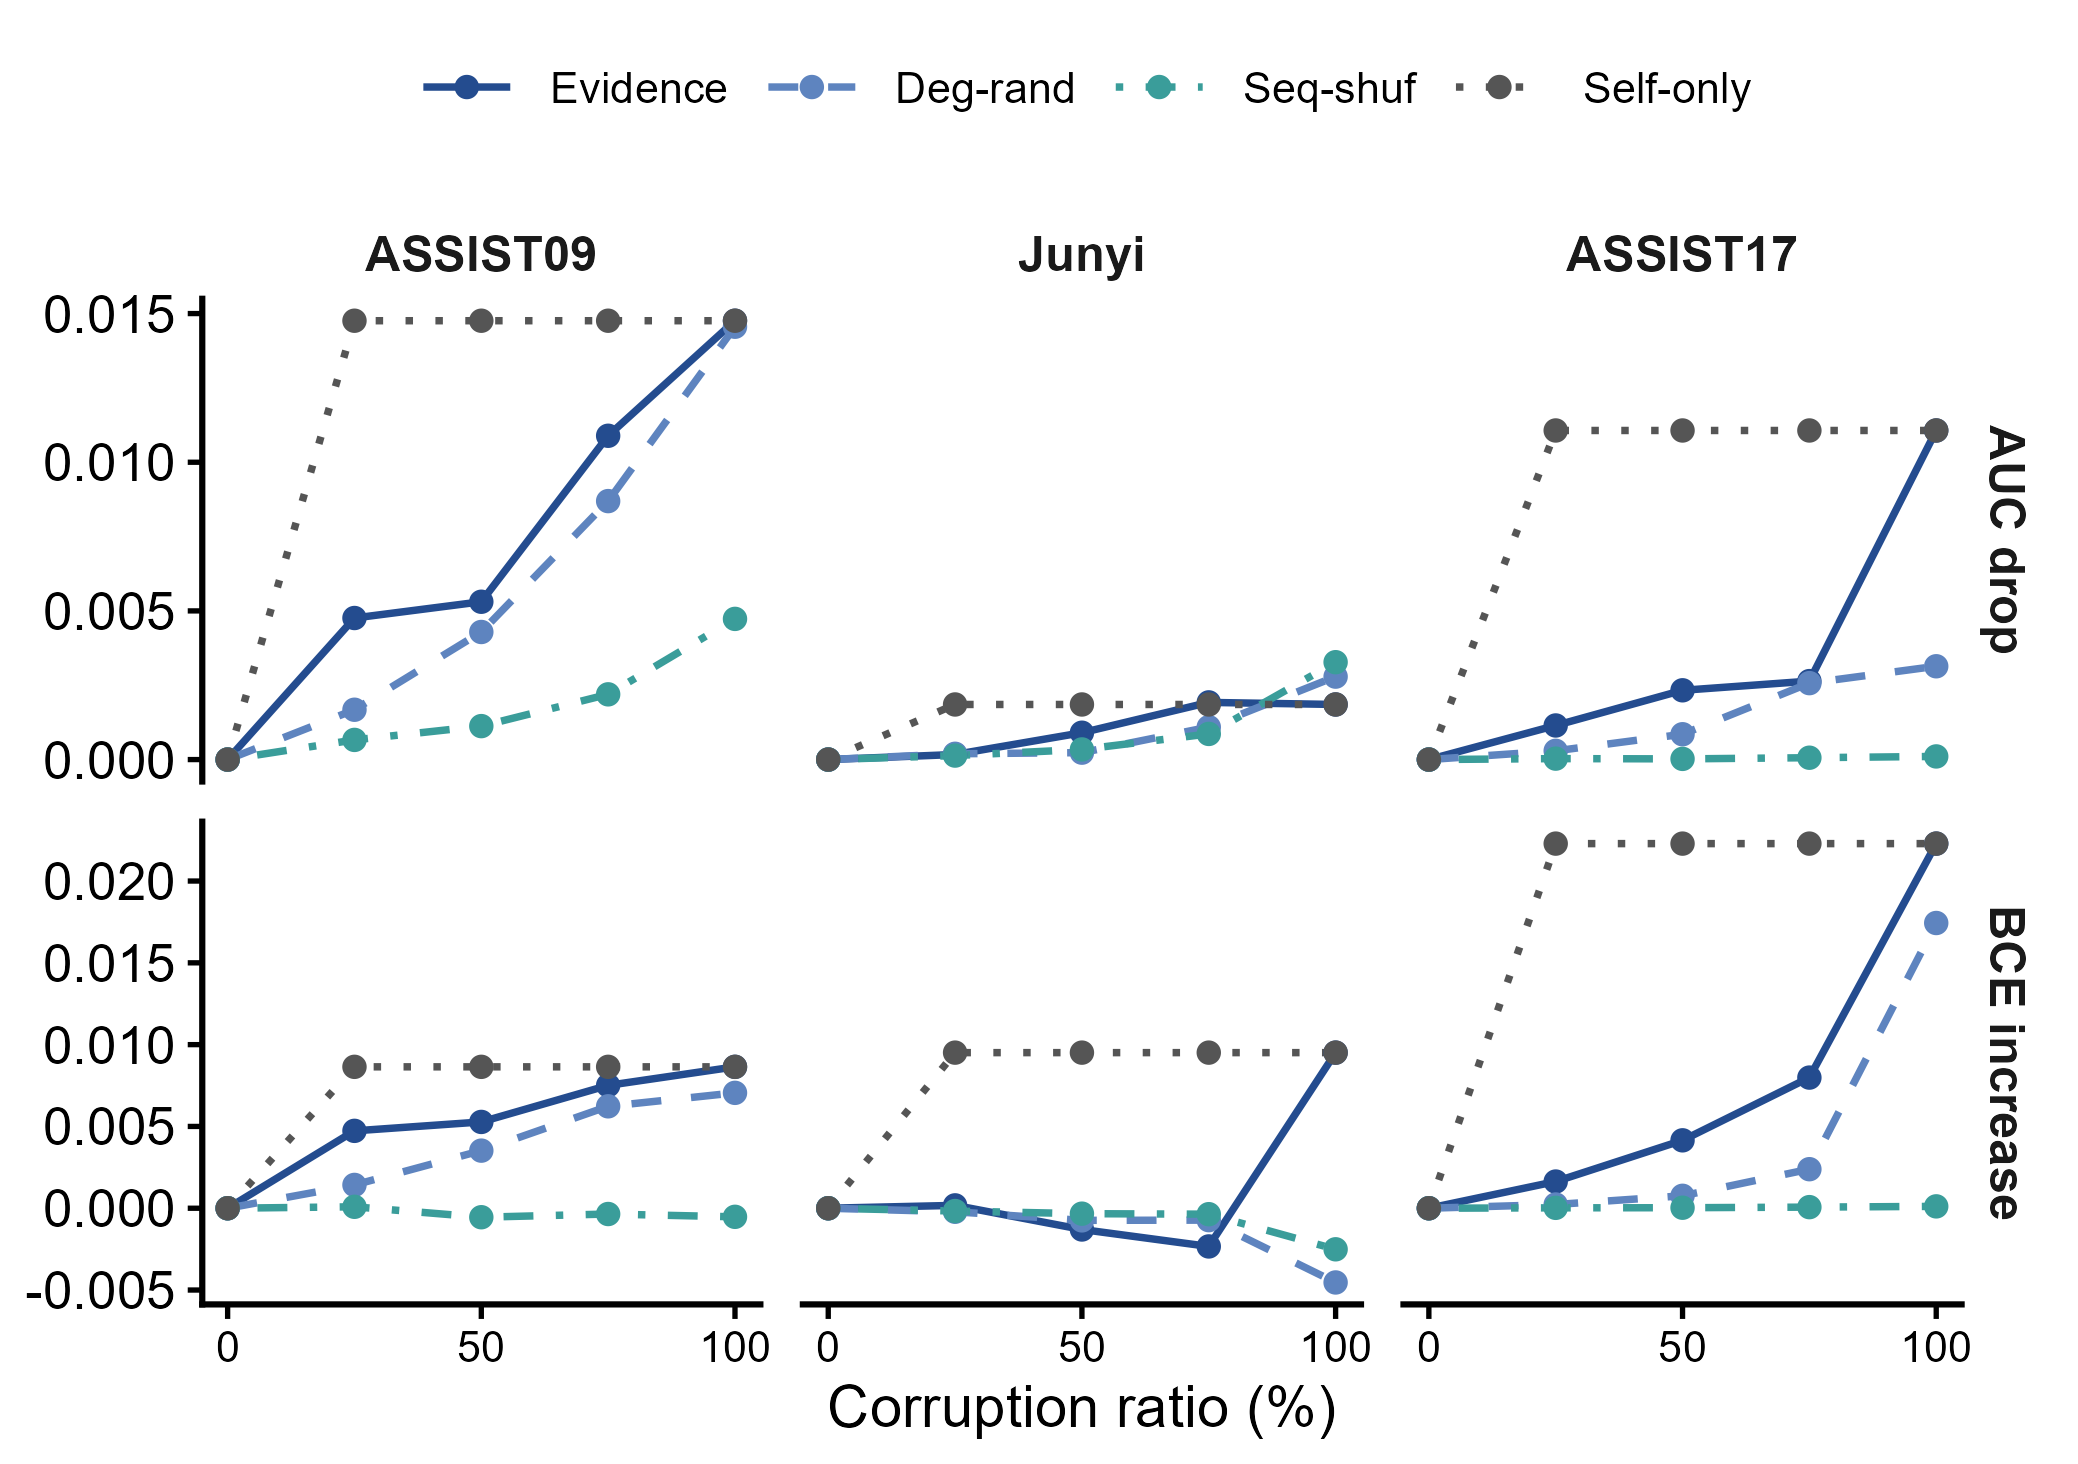
\includegraphics[width=0.98\columnwidth]{fig7_crg_support_perturbation.png}
  \caption{CRG 支持集扰动结果。上排为 AUC drop，下排为 BCE increase；曲线比较 evidence corruption、degree-random、sequence-shuffle 与 self-only fallback。}
  \label{fig:support-perturbation}
\end{figure}

图~\ref{fig:support-perturbation} 表明，替换 CRG 支持集会改变模型预测表现。ASSIST17 中证据支持集替换带来的变化大于度匹配随机支持集，说明模型对 CRG 支持概念具有较强依赖。ASSIST09 中证据替换与度匹配随机替换接近，体现出模型对候选支持空间的敏感性。Junyi 的 AUC 变化较小，但 BCE increase 显示支持集扰动会影响概率校准。

该结果补充了概念检索实验的另一侧面：CRG support 会影响训练后模型的预测行为。ASSIST17 中证据支持集替换的退化大于度匹配随机对照，说明模型对训练日志支持的候选概念更敏感；ASSIST09 更强调候选支持空间本身的重要性。不同数据集的表现差异也说明，CRG 更适合被解释为训练日志约束的概念支持，而非统一适用于所有数据分布的强先修图。

\subsection{学习者状态反事实与同题个案}
本节分析 LCRF 对学习者状态的使用方式。我们使用三种变体：no-filter 表示移除 LCRF；mean-state 用群体平均学生状态替代真实状态；shuffle-state 打乱学生状态。

\begin{figure}[H]
  \centering
  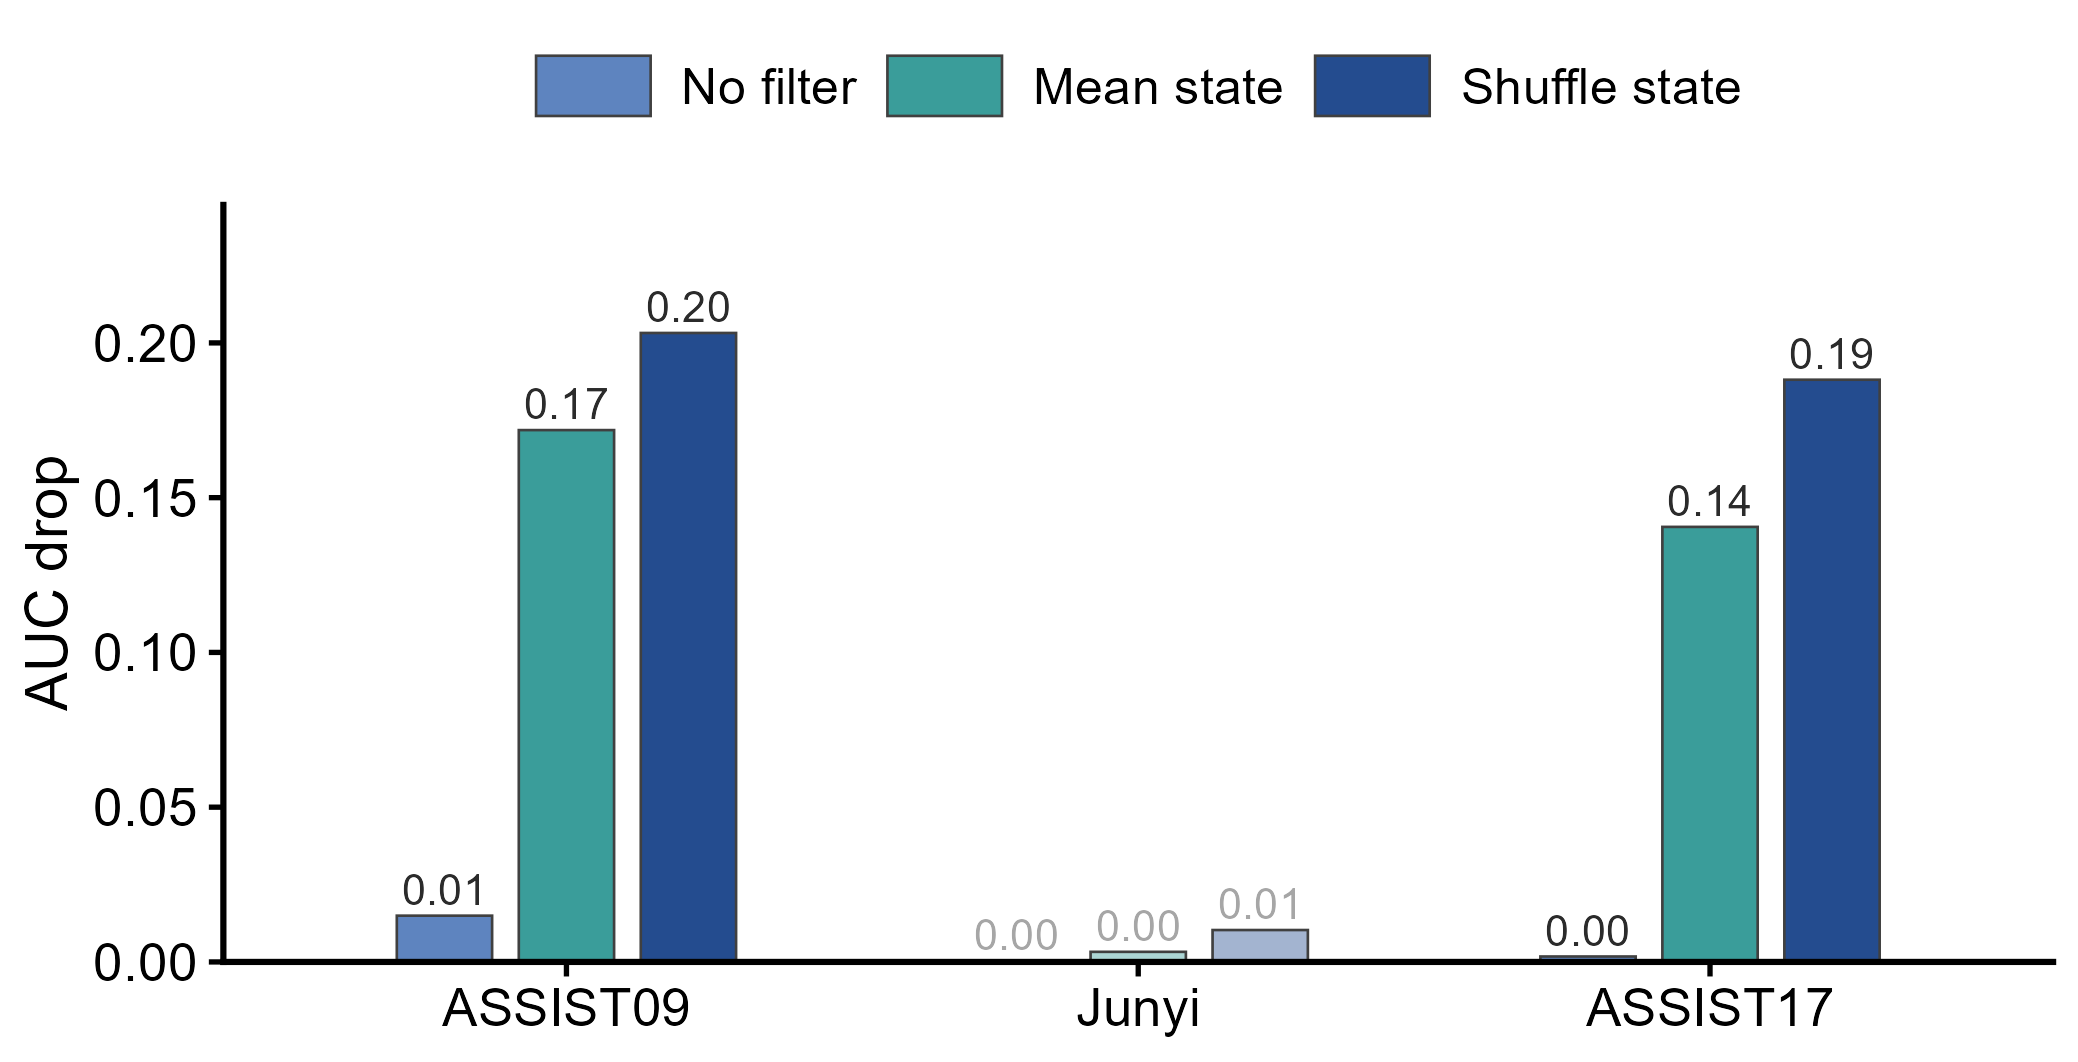
\includegraphics[width=0.98\columnwidth]{fig9_lcrf_counterfactual.png}
  \caption{LCRF 学习者状态反事实结果。图中比较 no-filter、mean-state 和 shuffle-state 相对完整模型的变化。}
  \label{fig:counterfactual}
\end{figure}

图~\ref{fig:counterfactual} 区分了模块移除和状态替换两类干预。no-filter 反映移除 LCRF 后的整体预测变化；mean-state 和 shuffle-state 进一步检验真实学习者状态是否可以由群体平均状态或错配状态替代。ASSIST09 和 ASSIST17 在 mean/shuffle 干预下出现明显下降，说明 LCRF 的后验分布依赖学习者状态。Junyi 的结果主要体现 CRG 的候选支持作用，LCRF 的状态替换效应不如 ASSIST09 和 ASSIST17 明显。

为了观察局部行为，本文固定同一个 query concept 和相同 CRG 支持集，比较不同学生得到的后验分布。ASSIST17 的主个案为 \texttt{ASSIST17\_Q14\_S25}。该个案中所有学生共享相同支持集，支持集大小为 25；候选统计显示 mean pairwise L1 最高可达到 0.801，JS 为 0.129。双学生对比中，S1 与 S7 的后验权重差异明显。

\begin{figure}[H]
  \centering
  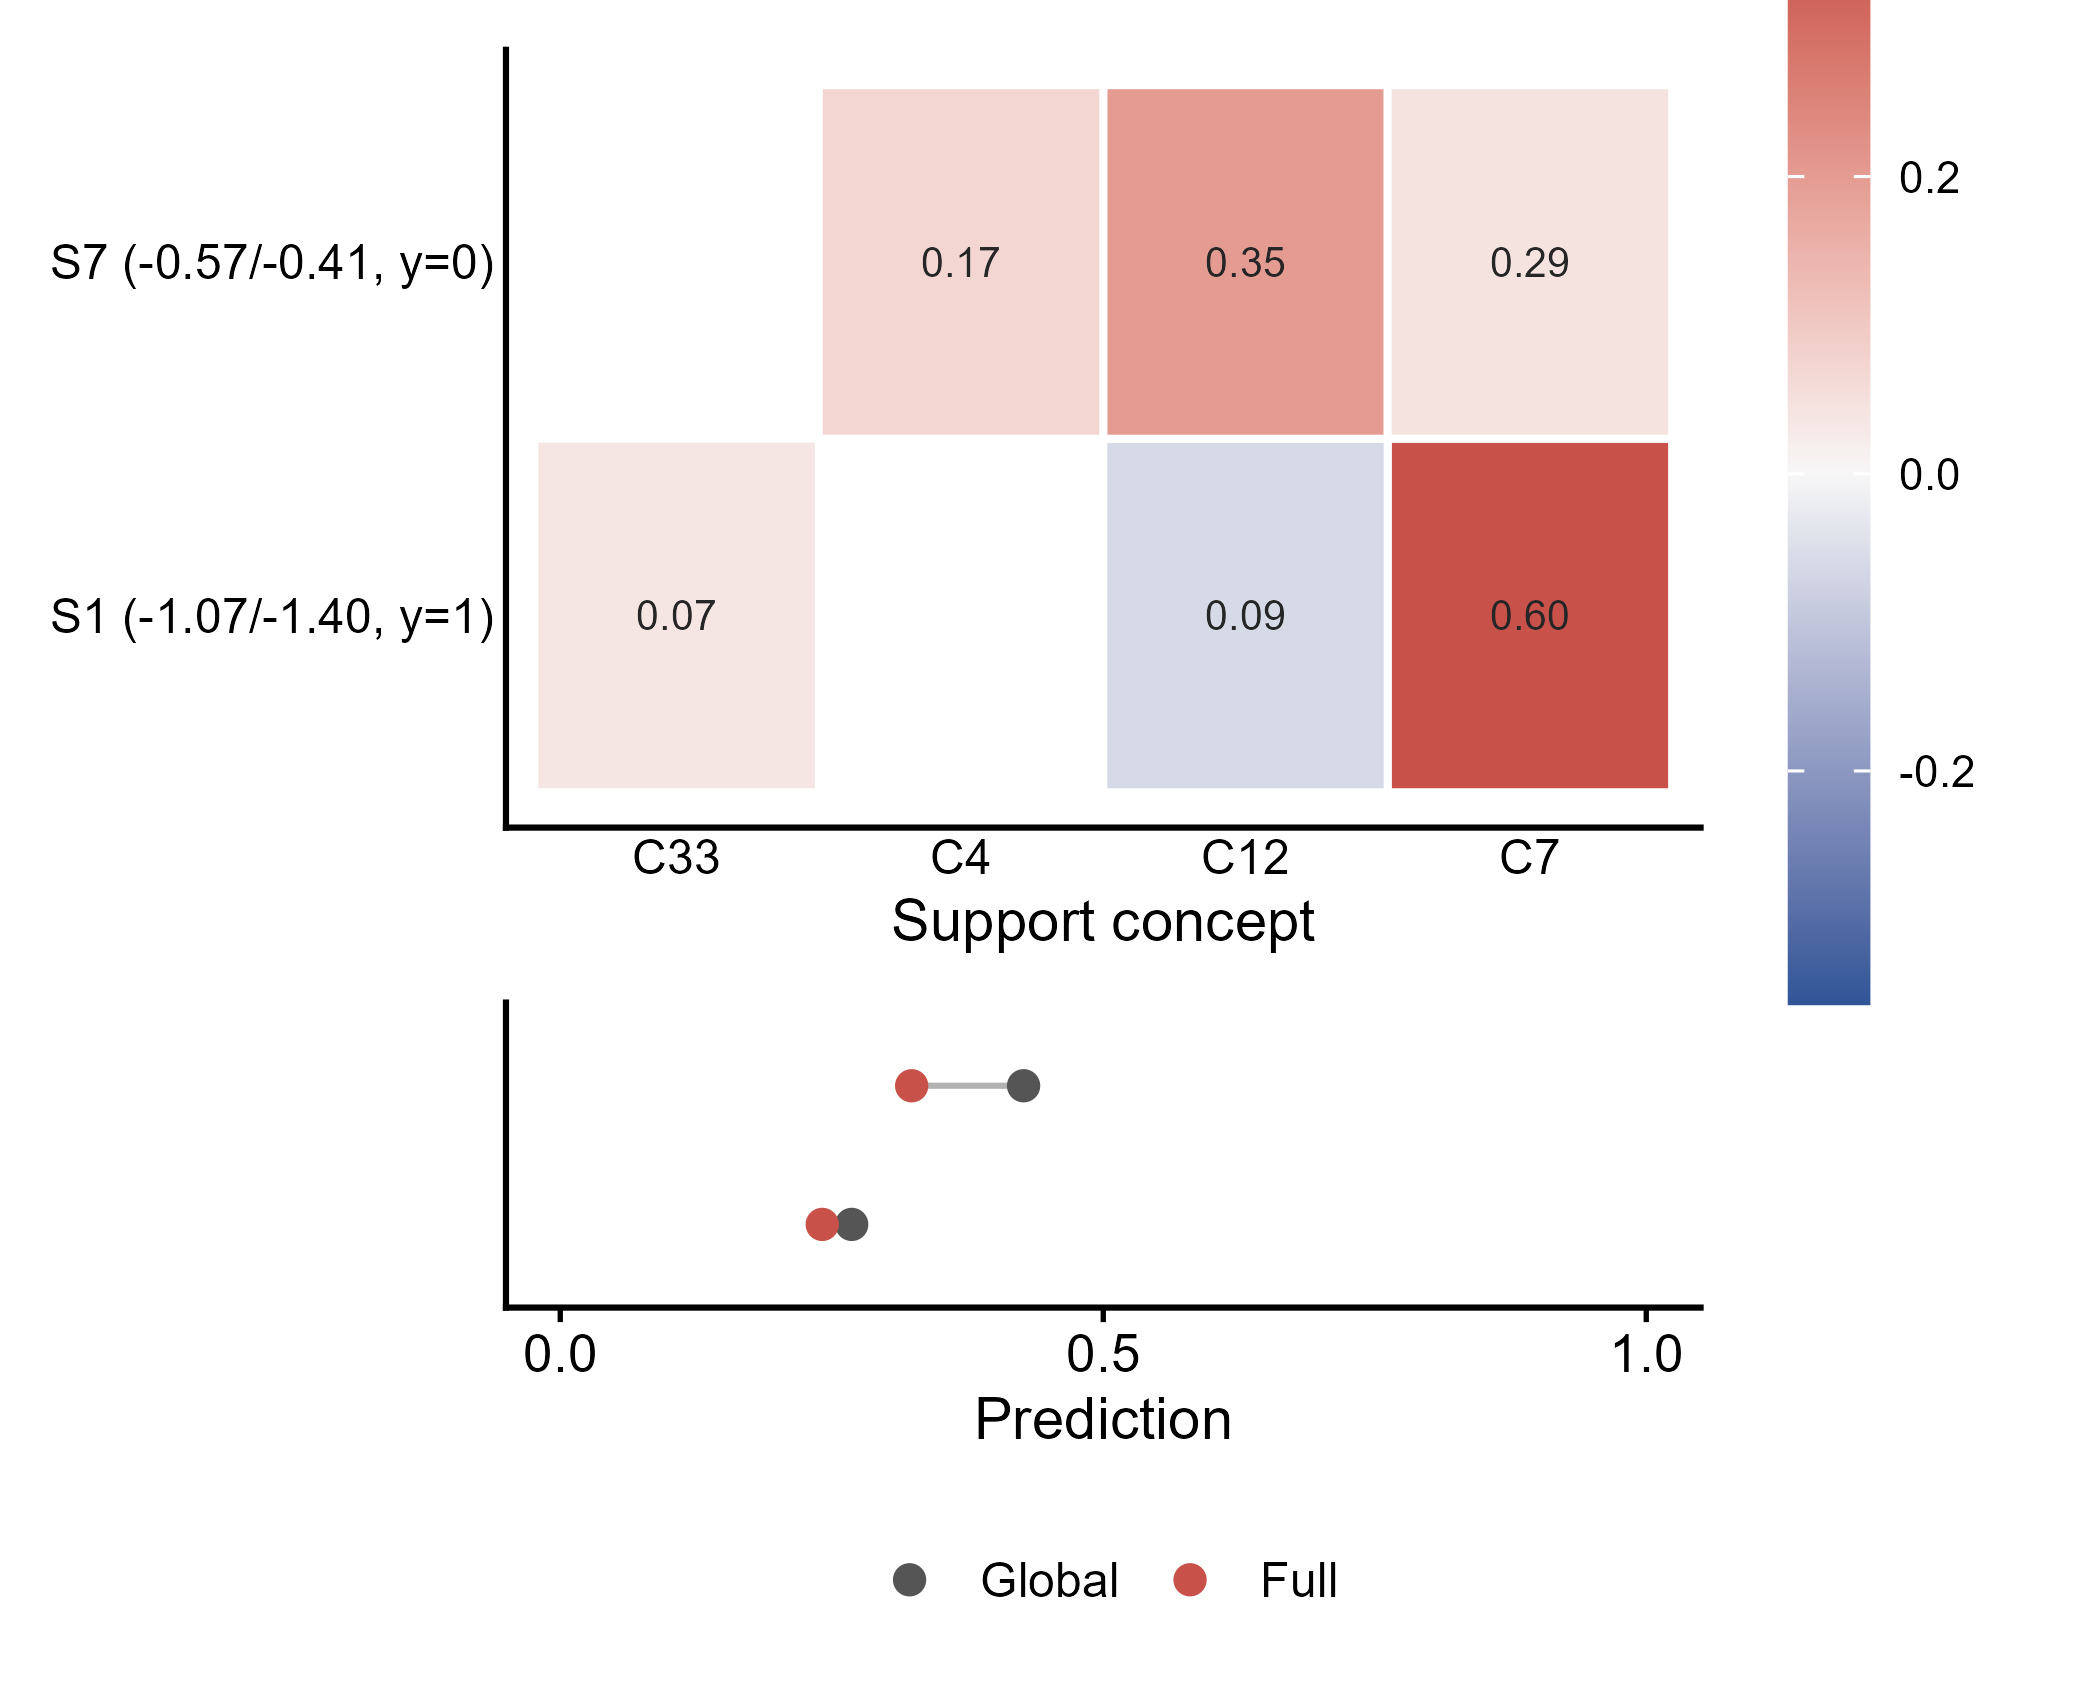
\includegraphics[width=0.98\columnwidth]{fig10_lcrf_same_query.png}
  \caption{同题后验个案。在同一 query concept 和同一 CRG 支持集下，不同学生获得不同支持概念后验权重。}
  \label{fig:same-query}
\end{figure}

图~\ref{fig:same-query} 展示了 LCRF 的个性化过滤行为：在同一 query、同一 CRG 支持集下，不同学生会得到不同后验分布。S1 的后验权重更集中于 C7，而 S7 更强调 C12；这说明 LCRF 在固定支持集内根据学习者状态调整支持概念权重。

这一结果对应 LCRF 的教育解释。CRG 给出的是全局可用支持，类似可供参考的候选学习线索；LCRF 根据学生 mastery、近期表现和历史计数对这些支持概念重新分配权重，使同一目标概念在不同学生上形成不同的局部支持权重。这里的后验变化不等同于教学干预，而是在预测层面体现“同一支持需要根据学生状态调整”的思想。

\section{局限性}
本文的序列关系来自训练日志中的经验转移，应解释为经验学习顺序而非严格课程先修关系。这一边界符合教育诊断中的基本直觉：当目标概念本身已有充分观测时，直接作答记录仍然是最具体的诊断信号。CRG/LCRF 应被视为直接历史作答不足时的补充支持，而不是直接概念状态的替代品。后续工作可以在更丰富的课程元数据和学习过程数据中进一步区分经验关系、课程结构和个体学习支架。

\section{结论}
本文提出面向概念证据缺口的 CRG-LCRF 框架。CRG 从训练阶段题内共现、序列转移和自保持关系中构造全局概念可达图，用于连接学生历史概念和当前目标概念；LCRF 在 CRG 固定支持集内，根据学生状态重排后验分布，实现支持约束的个性化过滤。

三个数据集上的实验表明，CRG 能在 ASSIST09 和 Junyi 上从学生历史概念中检索当前查询概念，并能恢复留出的概念转移。Coverage-conditioned prediction 进一步显示，CRG-LCRF 的预测收益主要出现在 ASSIST09 的 direct-unseen-bridgeable 子场景和 ASSIST17 的 high-score / 低直接覆盖子组中。支持集扰动、学习者状态反事实和同题个案分析分别展示了 CRG 支持集对预测的影响以及 LCRF 在固定支持集内的个性化过滤行为。该框架为目标概念缺少直接历史覆盖时的认知诊断提供了一种基于显式概念支持的建模方案。

\bibliographystyle{IEEEtran}
\bibliography{references_crg_lcrf}

\end{document}






